\documentclass[11pt, a4paper, abstract=true]{scrartcl}
\usepackage[sexy]{evan}
\usepackage{float}
\usepackage[margin=1.00in]{geometry}
\usepackage{multirow}
\usepackage{longtable}
\usepackage{chemformula}
\def\arraystretch{1.20}

% \clearpairofpagestyles
\setkomafont{pagenumber}{\itshape}
\KOMAoptions{}
\ohead{\footnotesize \textbf{\leftmark}}
\ihead{\footnotesize \textsc{Lab Report III}}
\cfoot{\pagemark}
\begin{document}
\subject{
    CH1202: Lab Report III
}
\title{
    \huge Determination of the \(pK_{\text{In}}\) value of an acid-base indicator by spectrophotometric method
}
\author{
    Abhisruta Maity \\
    {\normalsize 21MS006}
    \plusemail{am21ms006@iiserkol.ac.in}
}
\date{}
\publishers{
    \normalsize \emph{Indian Institute of Science Education and Research, Kolkata \\
    Mohanpur, West Bengal, 741246, India}
}
\maketitle

\tableofcontents

\section{Brief Theory and Equation}

Most of the acid-base indicator are technically weak acid (represented as HIn). In some solutions, it dissociates: \[\ch{HIn <=> H+ + In-}\] which yields the Henderson-Hasselbalch equation: \[pH = pK_{\text{In}} + \log{\frac{[\ch{In-}]}{[\ch{HIn}]}}\] Now to determine the ratio of \(\frac{[\ch{In-}]}{[\ch{HIn}]}\), we use spectrophotometry. We are acquainted with Beer's law: \[A = \epsilon cl\] where \(A\) is the absorbance of the solution, \(\epsilon\) being one of the intrisic property of the solution called the molar attenuation coefficient. We will find \(A\) at different \(pH\), which we lead to \(pK_\text{In}\) through Henderson-Hasselbalch equation. This requires a trick of using conservation of mass (since, \(m_{\ch{H+}} \ll m_{\ch{HIn}}\), we have \(m_{\ch{HIn}} \simeq m_{\ch{In-}}\)), as stated through the following equation (details were avoided): \[[\ch{HIn}] = \frac{A' - A}{\epsilon l}\] and \[[\ch{In-}] = \frac{A}{\epsilon l}\] plugging these back into the Henderson-Hasselbalch equation yields: \[pH = pK_{\text{In}} + \log{\frac{A}{A' - A}} \tag{\(\star\)}\] where \(A'\) is the absorbance of solution when HIn and \ch{In-} both are present in the solution and in equilibrium, while A denotes the absorbance of solution only \ch{In-} is present in the solution. The equation (\(\star\)) is the working formula for this experiment.

\section{Dataset}

% Please add the following required packages to your document preamble:
% \usepackage{multirow}
% Please add the following required packages to your document preamble:
% \usepackage{multirow}
% Please add the following required packages to your document preamble:
% \usepackage{multirow}
% Please add the following required packages to your document preamble:
% \usepackage{multirow}
% Please add the following required packages to your document preamble:
% \usepackage{multirow}
% Please add the following required packages to your document preamble:
% \usepackage{multirow}
% Please add the following required packages to your document preamble:
% \usepackage{multirow}
\begin{table}[H]
    \centering
    \begin{tabular}{|c|c|ccc|c|c|}
    \hline
    \begin{tabular}[c]{@{}c@{}}Sl.\\ No.\end{tabular} &
      \begin{tabular}[c]{@{}c@{}}Vol. of\\ Oxalic acid\\ (mL)\end{tabular} &
      \multicolumn{3}{c|}{\begin{tabular}[c]{@{}c@{}}Burette reading\\ (mL)\end{tabular}} &
      \begin{tabular}[c]{@{}c@{}}Avg. \\ Vol.\\ (mL)\end{tabular} &
      \begin{tabular}[c]{@{}c@{}}Strength of\\ NaOH\\ (N)\end{tabular} \\ \cline{3-5}
    \multicolumn{1}{|l|}{\multirow{2}{*}{}} &
      \multicolumn{1}{l|}{\multirow{2}{*}{}} &
      \multicolumn{1}{l|}{\multirow{2}{*}{Initial}} &
      \multicolumn{1}{l|}{\multirow{2}{*}{Final}} &
      \multicolumn{1}{l|}{\multirow{2}{*}{Difference}} &
      \multicolumn{1}{l|}{\multirow{2}{*}{}} &
      \multicolumn{1}{l|}{\multirow{2}{*}{}} \\
    \multicolumn{1}{|l|}{} &
      \multicolumn{1}{l|}{} &
      \multicolumn{1}{l|}{} &
      \multicolumn{1}{l|}{} &
      \multicolumn{1}{l|}{} &
      \multicolumn{1}{l|}{} &
      \multicolumn{1}{l|}{} \\ \hline
    1 &
      10 &
      \multicolumn{1}{c|}{0} &
      \multicolumn{1}{c|}{10} &
      10 &
      \multirow{3}{*}{10.1} &
      \multirow{3}{*}{0.5} \\ \cline{1-5}
    2 &
      10 &
      \multicolumn{1}{c|}{0} &
      \multicolumn{1}{c|}{10.2} &
      10.2 &
       &
       \\ \cline{1-5}
    3 &
      10 &
      \multicolumn{1}{c|}{0} &
      \multicolumn{1}{c|}{10.1} &
      10.2 &
       &
       \\ \hline
    \end{tabular}
    \caption{Standardization of NaOH solution with Oxalic acid}
    \end{table}

    % Please add the following required packages to your document preamble:
% \usepackage{multirow}
\begin{table}[H]
    \centering
    \begin{tabular}{|c|c|ccc|c|c|}
    \hline
    \begin{tabular}[c]{@{}c@{}}Sl.\\ No.\end{tabular} &
      \begin{tabular}[c]{@{}c@{}}Vol. of\\ Acetic acid\\ (mL)\end{tabular} &
      \multicolumn{3}{c|}{\begin{tabular}[c]{@{}c@{}}Burette reading\\ (mL)\end{tabular}} &
      \begin{tabular}[c]{@{}c@{}}Avg. \\ Vol.\\ (mL)\end{tabular} &
      \begin{tabular}[c]{@{}c@{}}Strength of\\ Acetic acid\\ (N)\end{tabular} \\ \cline{3-5}
    \multicolumn{1}{|l|}{\multirow{2}{*}{}} &
      \multicolumn{1}{l|}{\multirow{2}{*}{}} &
      \multicolumn{1}{l|}{\multirow{2}{*}{Initial}} &
      \multicolumn{1}{l|}{\multirow{2}{*}{Final}} &
      \multicolumn{1}{l|}{\multirow{2}{*}{Difference}} &
      \multicolumn{1}{l|}{\multirow{2}{*}{}} &
      \multicolumn{1}{l|}{\multirow{2}{*}{}} \\
    \multicolumn{1}{|l|}{} &
      \multicolumn{1}{l|}{} &
      \multicolumn{1}{l|}{} &
      \multicolumn{1}{l|}{} &
      \multicolumn{1}{l|}{} &
      \multicolumn{1}{l|}{} &
      \multicolumn{1}{l|}{} \\ \hline
    1 &
      10 &
      \multicolumn{1}{c|}{0} &
      \multicolumn{1}{c|}{10} &
      10 &
      \multirow{3}{*}{9.9} &
      \multirow{3}{*}{0.5} \\ \cline{1-5}
    2 &
      10 &
      \multicolumn{1}{c|}{11} &
      \multicolumn{1}{c|}{20.9} &
      9.9 &
       &
       \\ \cline{1-5}
    3 &
      10 &
      \multicolumn{1}{c|}{0} &
      \multicolumn{1}{c|}{9.9} &
      9.9 &
       &
       \\ \hline
    \end{tabular}
    \caption{Standardization of Acetic acid solution using standardized NaOH}
    \end{table}

    \begin{table}[H]
        \centering
        \begin{tabular}{|c|c|c|c|cccc|}
        \hline
        \begin{tabular}[c]{@{}c@{}}Test\\ tube\end{tabular} &
          \begin{tabular}[c]{@{}c@{}}Vol. of 0.4 N\\ Acetic acid\\ (mL)\end{tabular} &
          \begin{tabular}[c]{@{}c@{}}Vol. of 0.4 N\\ NaOH\\ (mL)\end{tabular} &
          \begin{tabular}[c]{@{}c@{}}Vol. of water\\ (mL)\end{tabular} &
          \multicolumn{1}{c|}{\begin{tabular}[c]{@{}c@{}}\(pH\)\\ (expt.)\end{tabular}} &
          \multicolumn{1}{c|}{\(A\)} &
          \multicolumn{1}{c|}{\(\lambda = \frac{A}{A' - A}\)} &
          \(\log(\lambda)\) \\ \hline
        1 & 5 & 0.5 & 4.5 & \multicolumn{1}{c|}{3.72} & \multicolumn{1}{c|}{0.0783} & \multicolumn{1}{c|}{0.1218}   & -0.9144 \\ \hline
        2 & 5 & 1.5 & 3.5 & \multicolumn{1}{c|}{4.27} & \multicolumn{1}{c|}{0.2469} & \multicolumn{1}{c|}{0.5221}   & -0.2835 \\ \hline
        3 & 5 & 2.5 & 2.5 & \multicolumn{1}{c|}{4.63} & \multicolumn{1}{c|}{0.3934} & \multicolumn{1}{c|}{1.2001}   & 0.0792  \\ \hline
        4 & 5 & 3.5 & 1.5 & \multicolumn{1}{c|}{4.99} & \multicolumn{1}{c|}{0.5168} & \multicolumn{1}{c|}{2.5284}   & 0.4028  \\ \hline
        5 & 5 & 4.5 & 0.5 & \multicolumn{1}{c|}{5.57} & \multicolumn{1}{c|}{0.7144} & \multicolumn{1}{c|}{105.0588} & 2.0214  \\ \hline
        6 & 0 & 2.5 & 7.5 & \multicolumn{4}{c|}{\(A' = 0.7212\)}                                                              \\ \hline
        \end{tabular}
        \caption{Spectrophotometric data}
        \end{table}

\section{Plots}

\begin{figure}[H]
  \centering
  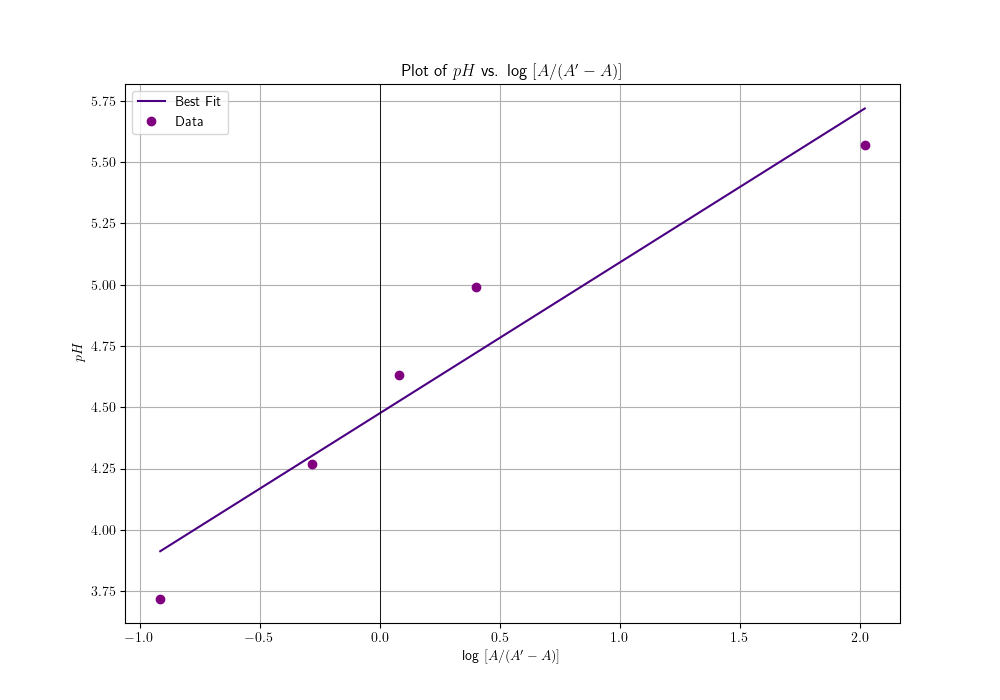
\includegraphics[scale=0.60]{plot.png}
  \caption{Fitting the experimented data}
\end{figure}

\section{Results}

From the above graph, by finding the \(y\)-intercept of the line we got by fitting (linear-regression) is \(pK_\text{In} = 4.48\), with a fitting error in intercept = \(2.26 \%\).

\end{document}